\overlays{2}{%
  \begin{slide}{Autogenerating Swarm Behaviors}
    Why autogenerate swarm behaviors?
    \fromSlide{1}{
      \begin{itemize}
      \item Trial-and-error gets tedious
      \item Complexity can quickly increase
      \item Emergence not always obvious
      \item Move away from low-level swarm programming
      \end{itemize}
    }
    \bigskip
    \fromSlide{2}{
      What is needed?
      \begin{itemize}
      \item Specify high-level goals
      \item Define lower-level behaviors, sensors, \ldots
      \item Use simulation to evaluate performance
      \end{itemize}
    }
  \end{slide}
}%

%%%%%
%%%%%

\begin{slide}{\ECS Overview}
  \vspace{.15\textheight}
  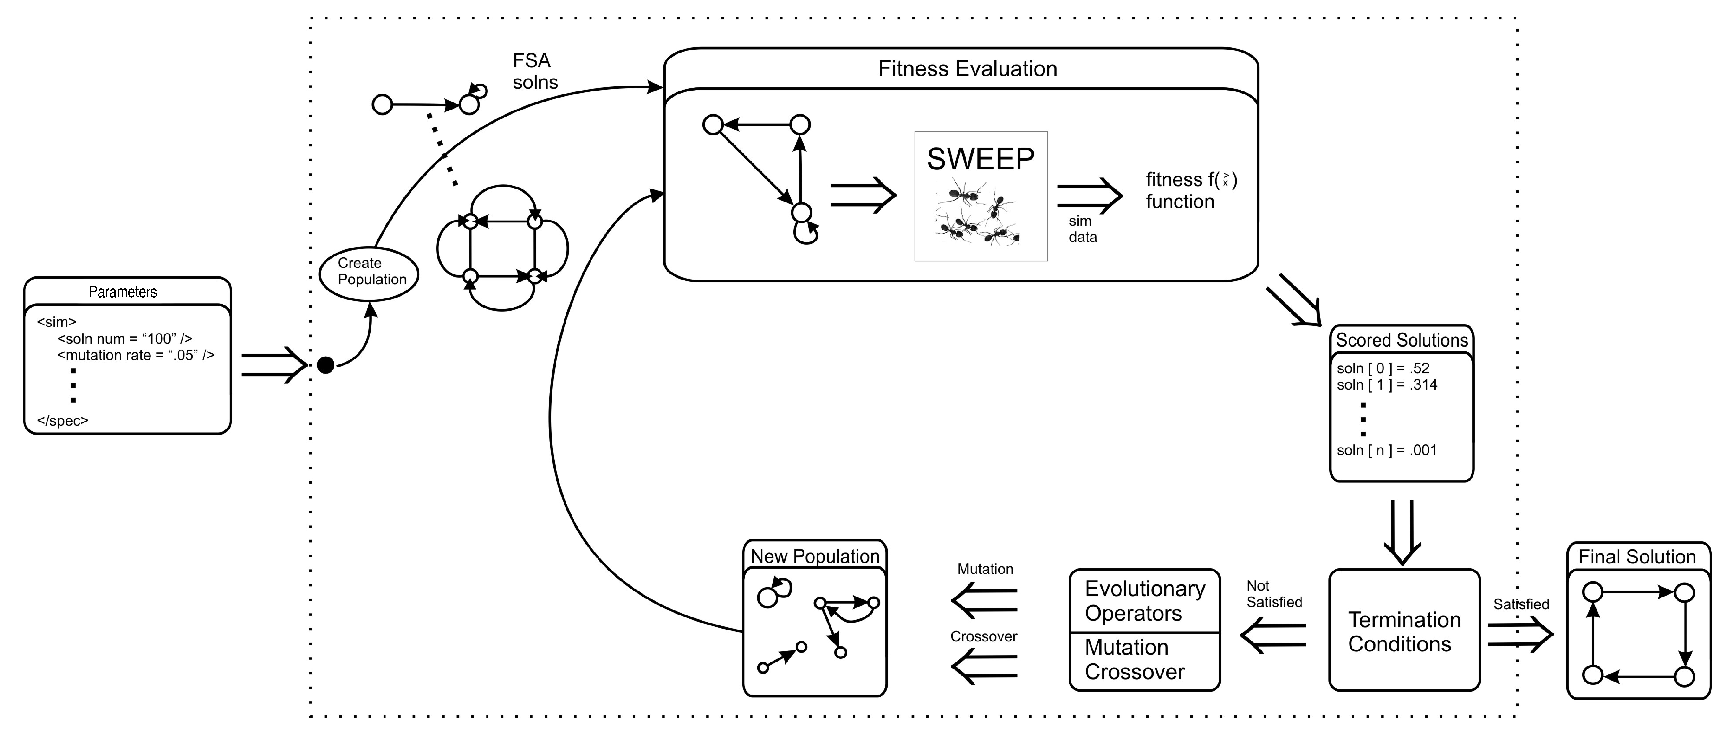
\includegraphics[scale=.4]{SystemOverview.eps}
\end{slide}

%%%%%
%%%%%

\begin{slide}{\ECS~- System Parameters}
  \centering
  \tiny
  \begin{tabular}{|lc|}
    \hline
    \multicolumn{2}{|c|}{\em{Parameters}} \\
    Objective & Dispersion \\
    Max. Generations & 500 \\
    Population Size  & 32  \\
    Number of Sims   & 2   \\	
    \hline
    \hline
    \multicolumn{2}{|c|}{\em{Mutations}}   \\
    Change-Sensor-Value & top 6 + 2 random \\
    Add-Transition      & top 6 + 2 random \\
    \hline
    \hline
    \em{Actions} & \em{Sensors}       \\
    move-random  & too-many neighbors \\
    move-none    & chemical-present   \\
    \hline
    \multicolumn{2}{|c|}{\em{Simulation}} \\
    Number of Agents & 100                \\
    Environment & $50 \times 50$ grid     \\
    \hline 
  \end{tabular}
\end{slide}

%%%%%
%%%%%

\begin{slide}{\ECS~- Solution Representation}
  \begin{minipage}{.65\textwidth}
    \SWEEP XML state machine
    \begin{itemize}
    \item Simple but expressive
    \item Graph-based
    \item Robust to random modification
    \end{itemize}
  \end{minipage}
  \hfill 
  \begin{minipage}{.3\textwidth}
    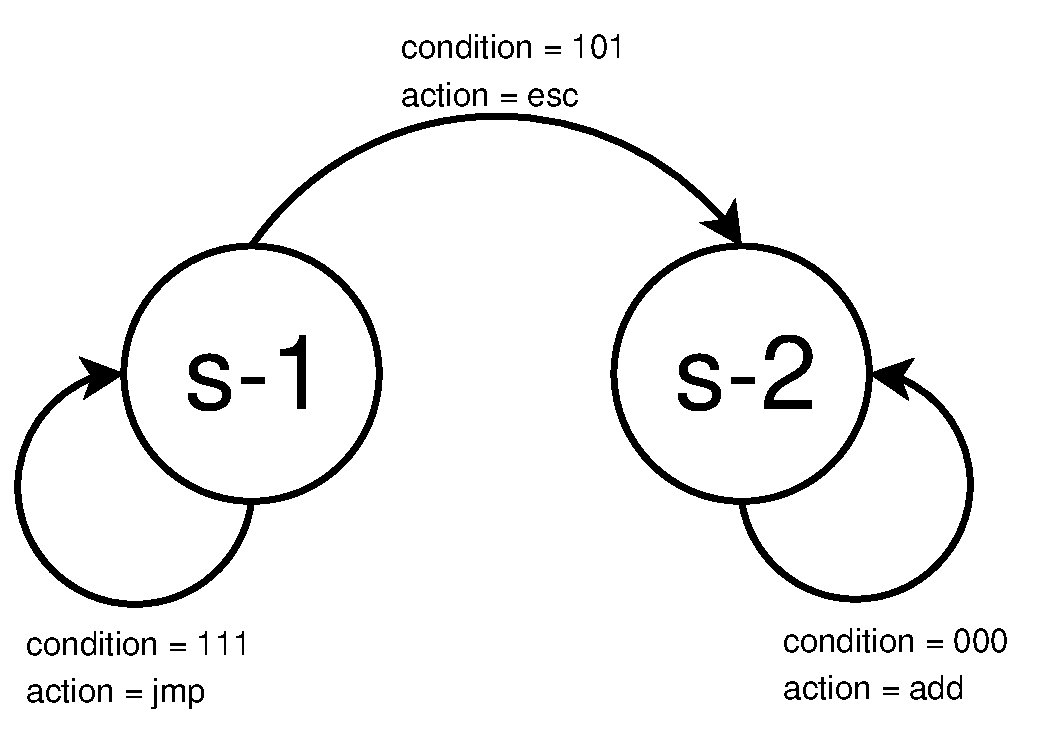
\includegraphics[scale=.2]{SimpleMachine}
  \end{minipage}\\
  \bigskip
  \bigskip
  \centering
  \begin{minipage}{.35\textwidth}
    \ttfamily
    \tiny
    \begin{tabbing}
      \hspace{1ex} \= \hspace{1ex} \= \hspace{1ex} \= \hspace{1ex} \= \hspace{2ex} \= \kill
      <states> \\
      \> <state name="A"> \\
      \> \> <transition nextState="s-1"> \\
      \> \> \> <sensor name="holding-object" value="true"/> \ldots \\
      \> \> \> <action name="jmp"/> \\
      \> \> </transition> \\
      \> </state> \\
      \> \vdots \\
    \end{tabbing}
  \end{minipage}
\end{slide}

%%%%%
%%%%%

\overlays{5}{%
\begin{slide}{\ECS~- Mutations}
  \vspace{2cm}
  \begin{minipage}{.45\textwidth}
    \begin{itemize}
    \item AddState
    \item AddTransition
    \item ChangeNextState
    \item InvertSensor
    \item ChangeAction
    \end{itemize}
  \end{minipage}
  \hfill
  %  \centering
  \begin{minipage}{.45\textwidth}
    \onlySlide*{1}{
      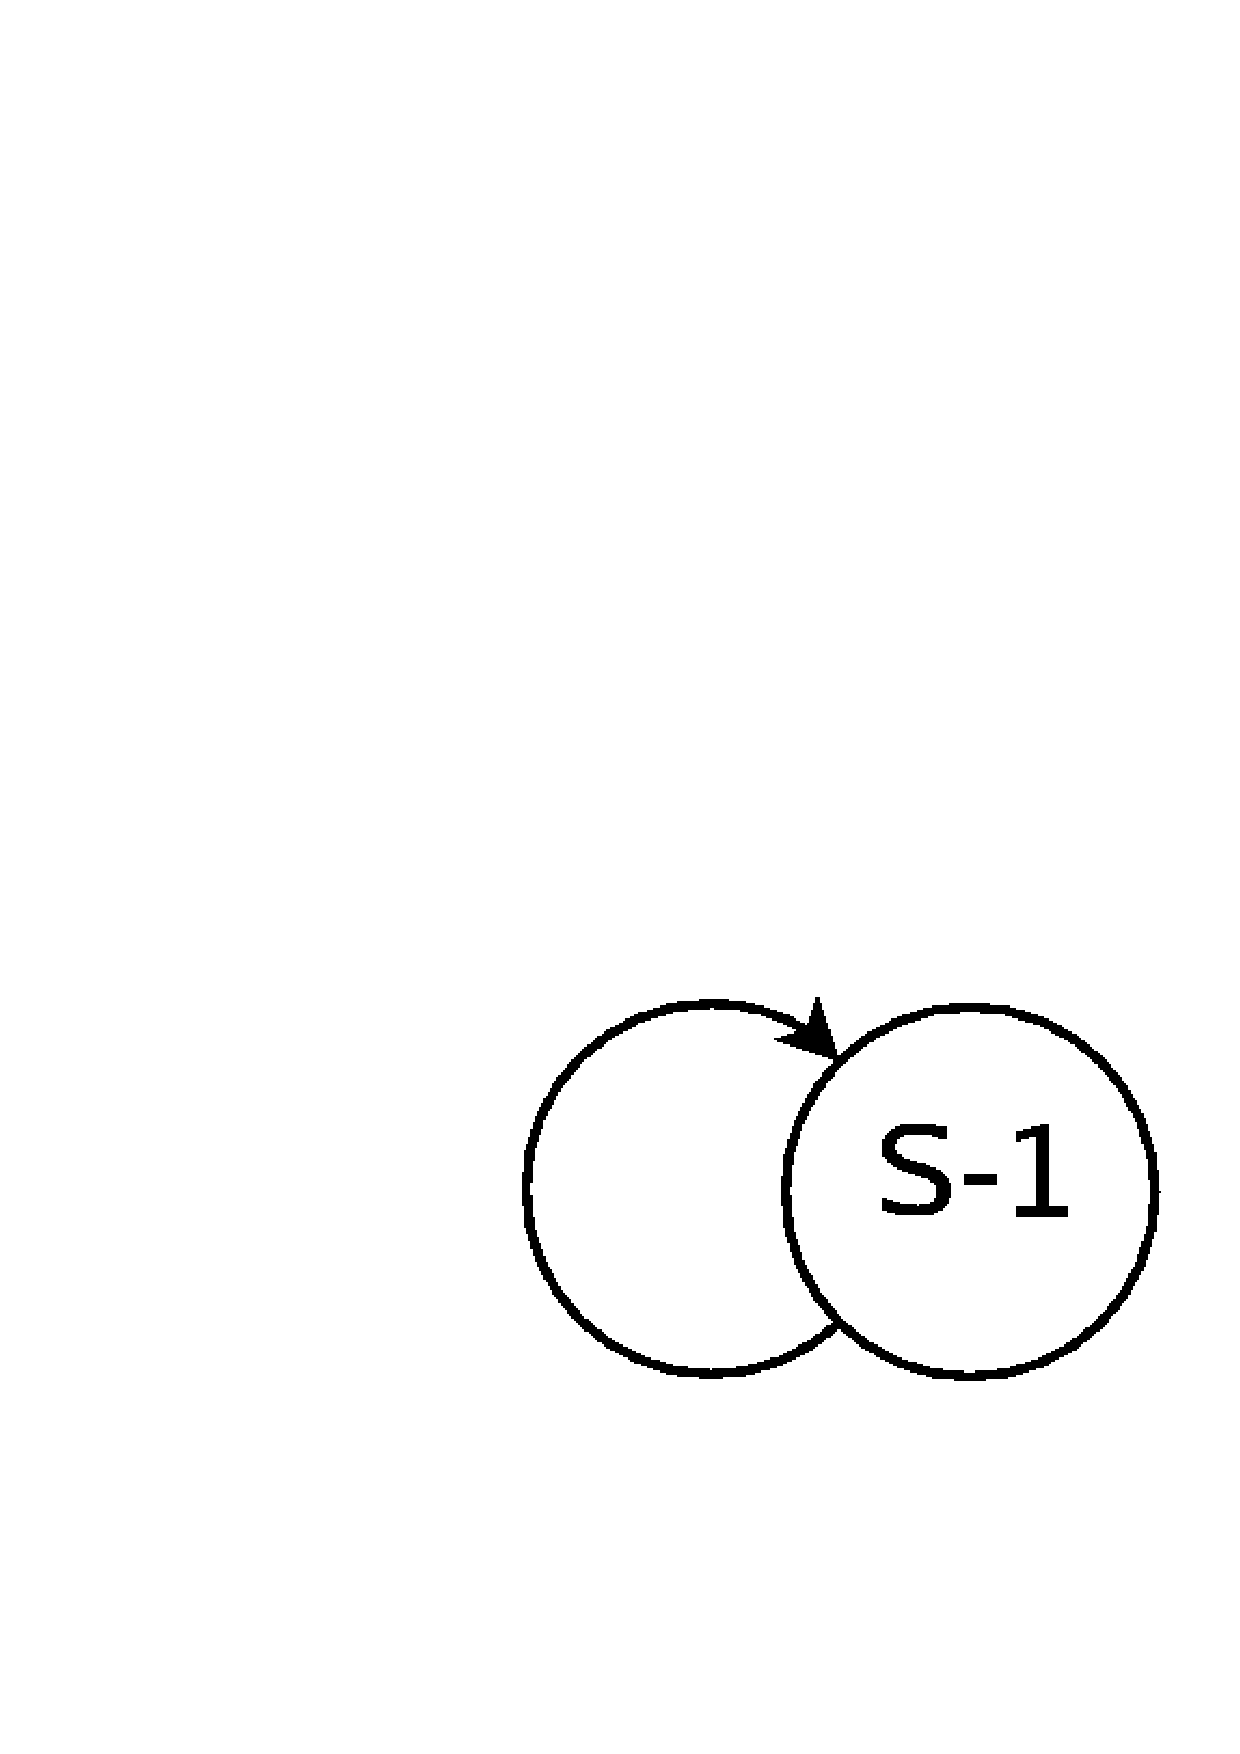
\includegraphics[scale=.25]{mutation0}
    }
    
    \onlySlide*{2}{
      % add state
      \includegraphics[scale=.25]{mutation1}
    }
    
    \onlySlide*{3}{
      % add transition
      \includegraphics[scale=.25]{mutation2}
    }
    
    \onlySlide*{4}{
      % change next state
      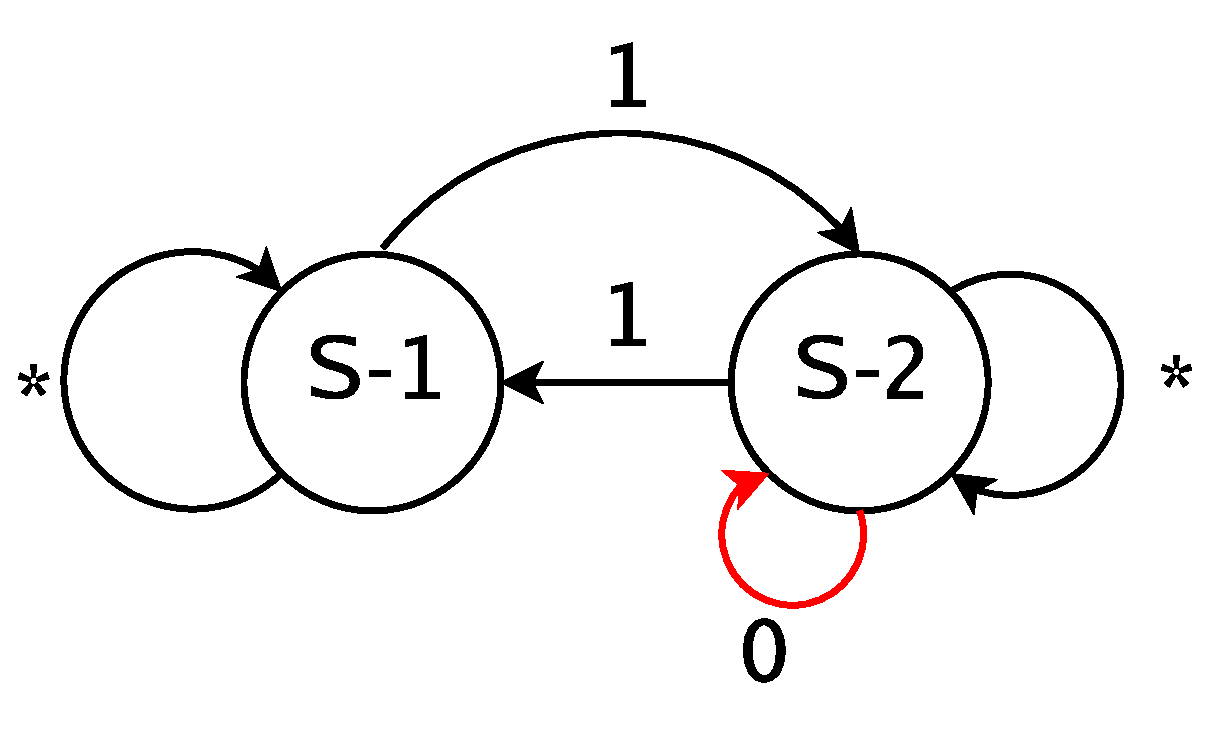
\includegraphics[scale=.25]{mutation3}
    }
    
    \onlySlide*{5}{
      % invert sensor
      \includegraphics[scale=.25]{mutation4}
    }
  \end{minipage}
\end{slide}
}

%%%%%
%%%%%

\begin{slide}{\ECS~- Fitness Evaluation}
  \begin{itemize}
  \item Differentiate good and bad solutions, imposes order
  \item Solutions simulated in \SWEEP
    \begin{itemize}
    \item One state machine solution $\rightarrow$ single agent program
    \item Homogeneous swarm
    \end{itemize}
  \item Multiple runs, remove biases
  \item Calculate fitness from raw \SWEEP output
  \item Error proportional to fitness, normalized
  \item Example
    
    \begin{tabular}{rlrl}
      \em{sweep}($s_1$) & = 7              & \em{sweep}($s_2$) & = 12             \\
      \em{error}($s_1$) & = 20-7 = 13      & \em{error}($s_2$) & = 20-12 = 8      \\
      \em{fitness}($s_1$) & = 13/20 = 0.65 & \em{fitness}($s_2$) & = 12/20 = 0.40 \\
      \multicolumn{4}{c}{\fbox{$s_2$ more fit}}
    \end{tabular}
  \end{itemize}
\end{slide}


